%document
\documentclass[10pt]{beamer}
%theme
\usetheme{metropolis}
% packages
\usepackage{color}
\usepackage{listings}
\usepackage[ngerman]{babel}
\usepackage[utf8]{inputenc}
\usepackage{multicol}

\usepackage{hyperref}
\hypersetup{colorlinks=true, linkcolor=blue, urlcolor=red}

% color definitions
\definecolor{mygreen}{rgb}{0,0.6,0}
\definecolor{mygray}{rgb}{0.5,0.5,0.5}
\definecolor{mymauve}{rgb}{0.58,0,0.82}

\lstset{
    backgroundcolor=\color{white},
    % choose the background color;
    % you must add \usepackage{color} or \usepackage{xcolor}
    basicstyle=\footnotesize\ttfamily,
    % the size of the fonts that are used for the code
    breakatwhitespace=false,
    % sets if automatic breaks should only happen at whitespace
    breaklines=true,                 % sets automatic line breaking
    captionpos=b,                    % sets the caption-position to bottom
    commentstyle=\color{mygreen},    % comment style
    % deletekeywords={...},
    % if you want to delete keywords from the given language
    extendedchars=true,
    % lets you use non-ASCII characters;
    % for 8-bits encodings only, does not work with UTF-8
    frame=single,                    % adds a frame around the code
    keepspaces=true,
    % keeps spaces in text,
    % useful for keeping indentation of code
    % (possibly needs columns=flexible)
    keywordstyle=\color{blue},       % keyword style
    % morekeywords={*,...},
    % if you want to add more keywords to the set
    numbers=left,
    % where to put the line-numbers; possible values are (none, left, right)
    numbersep=5pt,
    % how far the line-numbers are from the code
    numberstyle=\tiny\color{mygray},
    % the style that is used for the line-numbers
    rulecolor=\color{black},
    % if not set, the frame-color may be changed on line-breaks
    % within not-black text (e.g. comments (green here))
    stepnumber=1,
    % the step between two line-numbers.
    % If it's 1, each line will be numbered
    stringstyle=\color{mymauve},     % string literal style
    tabsize=4,                       % sets default tabsize to 4 spaces
    % show the filename of files included with \lstinputlisting;
    % also try caption instead of title
    language = C,
	showspaces = false,
	showtabs = false,
	showstringspaces = false,
	escapechar = ,
}

\def\ContinueLineNumber{\lstset{firstnumber=last}}
\def\StartLineAt#1{\lstset{firstnumber=#1}}
\let\numberLineAt\StartLineAt



\newcommand{\codeline}[1]{
	\alert{\texttt{#1}}
}

% This Document contains the information about this course.

% Authors of the slides
\author{
    Lecturers:
	%name1
	Mirko Jantschke,
	%name2
	Pascal Scholz
	\\
	%creaters of the slides
	Created by: Richard Mörbitz, Manuel Thieme
}


% Fancy Logo
\titlegraphic{\hfill
\includegraphics[height=1.25cm]{../templates/fsr_logo_cropped}}


\title{Dynamic storage}
\subtitle{Vol. 2}
\date{\today}

\usetikzlibrary{tikzmark}
\usetikzlibrary{arrows}
\usetikzlibrary{decorations.pathmorphing}
\tikzset{arrow/.style={-latex, shorten >=.5ex, shorten <=.5ex}}

% the actual document
\begin{document}

\maketitle

%-------------------------------------------------------------------------------------------------
\begin{frame}{Contents}
	\tableofcontents
\end{frame}

%-------------------------------------------------------------------------------------------------
\section{Rückblick - Wichtige Funktionen}
%-------------------------------------------------------------------------------------------------

\begin{frame}[fragile]{Ein kurzer Rückblick...}
Besonders große oder dynamische Datenstrukturen können und sollten auf dem Heap angelegt werden. Der unäre Operator \textit{sizeof} kann genutzt werden um die Größe von Objekten zu ermitteln. 
\\
\bigskip
Folgende Funktionen gibt es dafür in der \textit{stdlib.h}:
	\begin{itemize}
		\item \textit{malloc(size\_t size)}
		\item \textit{calloc(size\_t nitems, size\_t size)}
		\item \textit{realloc(void *ptr, size\_t size)}
		\item \textit{free(void *ptr)}
	\end{itemize}
\end{frame}

%-------------------------------------------------------------------------------------------------

\begin{frame}[fragile]{malloc()}
    \begin{lstlisting}[numbers=none]
void *malloc(size_t size);    \end{lstlisting}
Die Funktion malloc() 'fragt' beim Betriebssystem nach Speicher in der Größe von \textit{size} Bytes. Ist dies erfolgreich, wird ein Pointer auf den Anfang des Speicherbereiches zurückgegeben. Schlägt die Allokation fehl, wird ein \textit{NULL}-pointer zurückgeben. Der Speicher wird nicht initialisiert!
    \begin{lstlisting}[numbers=left]
/* Ein Beispiel */
 int *eineZahl = malloc(sizeof(*eineZahl));
 if(eineZahl != NULL) {
    *eineZahl = 3;
    /* Und noch viel mehr... */
 }\end{lstlisting}
\end{frame}

%-------------------------------------------------------------------------------------------------

\begin{frame}[fragile]{calloc()}
    \begin{lstlisting}[numbers=none]
void *calloc(size_t nitems, size_t size);    \end{lstlisting}
Erfüllt die selbe Funktion wie \textit{malloc()}, aber der Speicher wird mit dem Wert 0 initialisiert.
    \begin{lstlisting}[numbers=left]
/* Ein Beispiel */
 int *eineZahl = calloc(sizeof(*eineZahl));
 if(eineZahl != NULL) {
    printf("Ausgabe: %d\n", *eineZahl); // Ausgabe: 0
    /* Und noch viel mehr... */
 }\end{lstlisting}
\end{frame}

%-------------------------------------------------------------------------------------------------
\begin{frame}[fragile]{realloc()}
    \begin{lstlisting}[numbers=none]
void *realloc(void *ptr, size_t size);    \end{lstlisting}
Erfüllt die selbe Funktion wie \textit{malloc()}, wenn \textit{ptr == NULL} ist, sonst wird neuer Speicher in Größe von \textit{size} Bytes allokiert. Auf \textit{ptr} wird free aufgeführt, also nicht mehr verwenden! 
    \begin{lstlisting}[numbers=left]
/* Ein Beispiel */
 int *einArray = calloc(sizeof(*eineZahl));
 int *neu = realloc(eineZahl, 2 * sizeof(*neu));
 if(neu != NULL) {
    einArray = neu;     // Jetzt neu mit Platz fuer 2 integer
    einArray[0] = 1; 
    einArray[1] = 2;
    /* Und noch viel mehr... */
 }\end{lstlisting}
\end{frame}

%-------------------------------------------------------------------------------------------------
\begin{frame}[fragile]{free()}
    \begin{lstlisting}[numbers=none]
void free(void *ptr);    \end{lstlisting}
Gibt den mit \textit{malloc()}, \textit{calloc()} oder \textit{realloc()} auf dem Heap reservierten Speicher wieder frei. Der pointer \textit{ptr} sollte nicht mehr verwendet werden.
    \begin{lstlisting}[numbers=left]
/* Ein Beispiel */
 //Speicher wird allokiert
 int *eineZahl = calloc(sizeof(*eineZahl));
 if(eine != NULL) {
    /* Viel Code... */
    free(eineZahl); //Speicher wird freigegeben
 }
 return 0;\end{lstlisting}
\end{frame}

%---------------------------------------------------------------------------------------------------------------------------
\section{Die verkettete Liste - Ein Beispiel}

\begin{frame}[fragile]{Was wir vorhaben}
Nun wollen wir das Ganze an einem Beispiel ausprobieren.\\
\bigskip
Das Ziel: Wir wollen eine Datenstruktur bauen, mit der wir problemlos beliebig viele Zahlen speichern können. \\
\bigskip
Das Ganze werden wir nun Schritt für Schritt zusammen erarbeiten.
\end{frame}

%-------------------------------------------------------------------------------------------------

\begin{frame}[fragile]{Linked List - Konzept}
Eine verlinkte List, bzw linked list, speichert neben einem Element auch einen Verweis auf das nächste Element. Merkt man sich das Anfangselement, kann man alle anderen Elemente erreichen. Verliert man das erste Element, verliert man die gesamte Liste!
\\
\bigskip
\begin{figure}
 \centering
 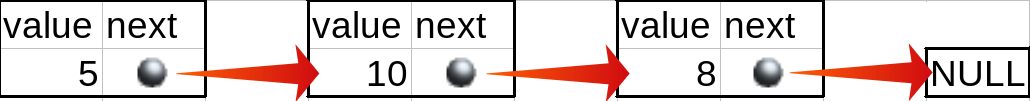
\includegraphics[width = \linewidth]{../img/stack_heap.png}
 \caption{Beweis, dass LibreOffice Calc ein vollwertiges Bildbearbeitungprogramm ist.}
 \label{figure:example}
\end{figure}


\end{frame}

%-------------------------------------------------------------------------------------------------

\section{Schritt 1 - Die Datenstruktur}
\begin{frame}[fragile]{Schritt 1 - Die Datenstruktur}
Wir benötigen eine Datenstruktur, welche einen Pointer auf das nächste Element der Liste und eine Zahl speichern kann.\\
\bigskip
\only<2->{
    Wir benutzen ein Struct!
}
\bigskip

\begin{onlyenv}<2->
\begin{lstlisting}[numbers=none]
struct list_elemnt {
    /* ?? */
};
\end{lstlisting}
\end{onlyenv}

\end{frame}

%-------------------------------------------------------------------------------------------------
\begin{frame}[fragile]{Schritt 1 - Die fertige Datenstruktur}
Diese Struktur könnne wir verwenden:\\
\bigskip
\begin{lstlisting}[numbers=left]
struct list_element {
    int value;
    struct list_element *next;
};
\end{lstlisting}
\end{frame}

%-------------------------------------------------------------------------------------------------

\section{Schritt 2 - Verwenden der Datenstruktur und Einfügen}

%-------------------------------------------------------------------------------------------------
\begin{frame}[fragile]{Schritt 2 - Wir erzeugen 2 Elemente zum Testen}
Wir können nun zwei Elemente unserer Struktur erzeugen um diese zu testen. Diese legen wir auf dem Heap an, da unsere Liste später einmal dynamisch wachsen soll.
\bigskip
\begin{lstlisting}[numbers=left]
int main(void) {
    struct list_element *list = malloc(sizeof(*a));
    struct list_element *newEntry = malloc(sizeof(*b));
    return 0;
}
\end{lstlisting}
\end{frame}

%-------------------------------------------------------------------------------------------------

\begin{frame}[fragile]{Schritt 2 - Wertezuweisung}
Diesen sollten Werte zugewiesen werden..
\bigskip
\begin{lstlisting}[numbers=left]
int main(void) {
    struct list_element *list;
    /* Zuweisung */
    return 0;
}
\end{lstlisting}

\end{frame}

%-------------------------------------------------------------------------------------------------
\begin{frame}[fragile]{Schritt 2 - Wertezuweisung}
Diesen sollten nun Werte zugewiesen werden...
\bigskip
\begin{lstlisting}[numbers=left]
int main(void) {
    struct list_element *list;
    struct list_element *newEntry;
    list->value = 10;
    list->value = NULL;
    /* Analog fuer newEntry */
    return 0;
}
\end{lstlisting}

\end{frame}

%-------------------------------------------------------------------------------------------------
\begin{frame}[fragile]{Schritt 2 - Wertezuweisung}
Jetzt können wir beide Elemente verketten. \\
\bigskip
Doch wie?
\end{frame}

%-------------------------------------------------------------------------------------------------

\begin{frame}[fragile]{Schritt 2 - Wertezuweisung}
Jetzt können wir beide Elemente verketten. \\
\bigskip
... indem wir den Pointer setzen!
\begin{lstlisting}[numbers=left]
int main(void) {
    struct list_element *list;
    struct list_element *newEntry;
    /* Code */
    list->next = newEntry;
    /* Code */
}\end{lstlisting}

\end{frame}

%-------------------------------------------------------------------------------------------------
\section{Schritt 3 - Die Liste ausgeben}
%-------------------------------------------------------------------------------------------------

\begin{frame}[fragile]{Schritt 3 - Die Ausgabe}
Nun haben wir eine Liste mit zwei Elementen. Wir können diese natürlich nun wie folgt jeweils ausgeben: \\
\begin{lstlisting}[numbers=left]
int main(void) {
    struct list_element *list;
    struct list_element *newEntry;
    /* Code */
    printf("Element 1: %d", list->value);
    printf("Element 2: %d", list->next->value);
    /* Code */
}\end{lstlisting}
Wenn wir aber mehr als zwei Elemente in unserer Liste haben und das für jedes Element machen müssten, würde diese Lösung schnell unpraktisch werden.

\end{frame}

%-------------------------------------------------------------------------------------------------

\begin{frame}[fragile]{Schritt 3 - Die Schleife...}
Schlauer ist es dafür eine Schleife anzulegen: \\
\begin{lstlisting}[numbers=left]
int main(void) {
    /* Code */
    /* Dies ist eine Luecke */
    while (/* Luecke */) {
        printf("Element: %d", /* Luecke */);
        /* Luecke */
    }
    /* Code */
}\end{lstlisting}
\end{frame}

%-------------------------------------------------------------------------------------------------
\begin{frame}[fragile]{Schritt 3 - Die Schleife}
Schlauer ist es dafür eine Schleife anzulegen: \\
\begin{lstlisting}[numbers=left]
int main(void) {
    /* Code */
    struct list_element *elem = list;
    while (/* Luecke */) {
        printf("Element: %d", /* Luecke */);
        /* Luecke */
    }
    /* Code */
}\end{lstlisting}
\end{frame}

%-------------------------------------------------------------------------------------------------

\begin{frame}[fragile]{Schritt 3 - Die Schleife...}
Schlauer ist es dafür eine Schleife anzulegen: \\
\begin{lstlisting}[numbers=left]
int main(void) {
    /* Code */
    struct list_element *elem = list;
    while (elem != NULL) {
        printf("Element: %d", /* Luecke */);
        /* Luecke */
    }
    /* Code */
}\end{lstlisting}
\end{frame}

%-------------------------------------------------------------------------------------------------

\begin{frame}[fragile]{Schritt 3 - Die Schleife...}
Schlauer ist es dafür eine Schleife anzulegen: \\
\begin{lstlisting}[numbers=left]
int main(void) {
    /* Code */
    struct list_element *elem = list;
    while (elem != NULL) {
        printf("Element: %d", /* Luecke */);
        elem = elem->next;
    }
    /* Code */
}\end{lstlisting}
\end{frame}

%-------------------------------------------------------------------------------------------------

\begin{frame}[fragile]{Schritt 3 - Die Schleife...}
Schlauer ist es dafür eine Schleife anzulegen: \\
\begin{lstlisting}[numbers=left]
int main(void) {
    /* Code */
    struct list_element *elem = list;
    while (elem != NULL) {
        printf("Element: %d", elem->value);
        elem = elem->next;
    }
    /* Code */
}\end{lstlisting}

Wenn wir unsere Liste mehrmals ausgeben wollen, bietet es sich an, diese Schleife in eine Funktion auszulagern.
\end{frame}

%-------------------------------------------------------------------------------------------------

\begin{frame}[fragile]{Schritt 3 - ...ausgelagert in eine Funktion}
\begin{lstlisting}[numbers=left]
void printList(struct list_element *begin) {
    while (begin != NULL) {
        printf("Element: %d", begin->value);
        begin = begin->next;
    }
}

int main(void) {
    struct list_element *list;
    /* Code */
    printList(list);
    /* Code */
}
\end{lstlisting}
Der Pointer \textit{begin} ist dabei eine lokale Kopie der übergebenen Adresse. Solange wir diesen nicht derefierzieren (mit *begin), wird \textit{list} nicht überschrieben.
\end{frame}
 
%-------------------------------------------------------------------------------------------------
\section{Schritt 4 - Auslagern des Einfügens}
%-------------------------------------------------------------------------------------------------

\begin{frame}[fragile]{Schritt 4 - Das Einfügen wird...}
Nun möchten wir beim Einfügen eines neuen Elementes dieses nicht immer von Hand verlinken.
\begin{lstlisting}[numbers=left]
int main(void) {
    /* Code */
    struct list_element *last = /* Das letzte Element von list*/;
    struct list_element *new = malloc(sizeof(*new));
    new->value = 24;
    new->next  = NULL;
    last->next = new;
    /* Code */
}
\end{lstlisting}
\end{frame}
 
%-------------------------------------------------------------------------------------------------
\begin{frame}[fragile]{Schritt 4 - ...ebenfalls ausgelagert}
Das könnte wie folgt aussehen:
\begin{lstlisting}[numbers=left]
void append(struct list_element *begin, int value) {
    /* Code */
}

int main(void) {
    /* Code */
    struct list_element *list = malloc(sizeof(*list));
    /* Code*/
    append(list, 24);
    /* Code */
}
\end{lstlisting}
\end{frame}
 
%-------------------------------------------------------------------------------------------------

\section{Aufgaben}
%-------------------------------------------------------------------------------------------------
\begin{frame}[fragile]{Vervollstädigung append()}
Die Funktion \textit{append()} soll ein neues \textit{list\_element} am Ende der Liste einfügen. Der Wert, der im neuen Element gespeichert wird, soll \textit{value} sein.
\begin{lstlisting}[numbers=left]
void append(struct list_element *begin, int value) {
    /* Code */
}
\end{lstlisting}
Zusatz: Verändere die Datenstruktur so, dass das Einfügen am Ende schneller wird. Eventuell sind dafür auch Anpassungen an den anderen Funktionen nötig.
\end{frame}
 
%-------------------------------------------------------------------------------------------------

\begin{frame}[fragile]{Einfügen nach Index}
Die Funktion \textit{insert()} soll ein neues \textit{list\_element} an der Stelle \textit{index} der Liste einfügen. Der Wert, der im neuen Element gespeichert wird, soll \textit{value} sein.
\begin{lstlisting}[numbers=left]
void insert(struct list_element *begin, int value, size_t index) {
    /* Code */
}
\end{lstlisting}
Zum Beispiel soll in die Liste 1-2-3-4 und \textit{index} == 2 und \textit{value} == 24 der Wert 24 zwischen die 1 und die 2 eingefügt werden, also 1-24-2-3-4.\\
ACHTUNG: Es müssen Randfälle beachtet werden.
\end{frame}
 
%-------------------------------------------------------------------------------------------------
\end{document}
